\documentclass[conference]{IEEEtran}
\IEEEoverridecommandlockouts
% The preceding line is only needed to identify funding in the first footnote. If that is unneeded, please comment it out.
\usepackage[
backend=biber,
style=numeric,
sorting=none
]{biblatex}
\addbibresource{bibliography.bib}
\usepackage{amsmath,amssymb,amsfonts}
\usepackage{algorithmic}
\usepackage{enumitem}
\usepackage{graphicx}
\usepackage{textcomp}
\usepackage{xcolor}
\usepackage{pgfplots}
\pgfplotsset{compat=1.16}
\def\BibTeX{{\rm B\kern-.05em{\sc i\kern-.025em b}\kern-.08em
    T\kern-.1667em\lower.7ex\hbox{E}\kern-.125emX}}
\begin{document}

\title{Extended Measurements of Centralization in Ethereum}

\author{\IEEEauthorblockN{Simon Brown}
\IEEEauthorblockA{\textit{ConsenSys Software Inc.}\\
simon.brown@consensys.net}
}

\maketitle

\begin{abstract}
Ethereum is undergoing significant changes to it's architecture as it evolves.  These changes include it's switch to PoS consensus and the introduction of significant infrastructural changes that do not require a change to the core protocol, but that fundamentally affect the way users interact with the network.  These changes represent an evolution toward a more modular architecture, in which have emerged new exogenous vectors for centralization.  This paper builds on previous models for measuring the level of decentralization of Ethereum that reflects these recent significant changes and Ethereum's new modular paradigm.
\end{abstract}

\begin{IEEEkeywords}
blockchain, Ethereum, decentralization, cryptocurrency, cryptoeconomics, web3
\end{IEEEkeywords}

\section{Introduction}

As web3 and cryptocurrencies are a relatively nascent socio-technological innovation, the broader ecosystem is in a phase of initial rapid innovation in which the architecture and topology of the networks are evolving significantly.  This is a well understood phenomenon in technological innovation, which was documented as early as the 1960s \cite{rogers2010diffusion}, in which the innovation and adoption of new technologies progress in an “S-Curve” shape, involving compressed stages of very rapid innovation followed by a period where innovation plateaus for a time.  Ethereum is an example of a technology that is in the rapid innovation phase, in which there are significant changes to the topology of the overall network, both intrinsic and extrinsic to the core protocol.

Previous research \cite{gochhayat2020measuring, lin2021measuring, karakostas2022sok} focused on measuring decentralization at the various layers of a vertical stack within a monolithic system.  The contribution of this paper is a model for measuring decentralization that adapts previous models to Ethereum's contemporary ecosystem topology.

The paper is organized as follows: in the background section we deliver an overview of how Ethereum is evolving and the challenge faced when attempting the measure it's level of decentralization.  In section III we outline the various dimensions that we propose to measure within model.  In section IV we describe our methodology, including the various indices that are applied to our data, and are data sources.  Section V we deliver a breakdown of results, and we close with our conclusions in section VI.

\section{Background}

It can be argued that protocols that are built on top of the base layer of Ethereum do not pose a direct threat to the base layer itself, even when they are highly centralized, and should therefore not be a factor in quantifying the network's level of decentralization.  Once the base layer is sufficiently decentralized, any number of protocol designs can be implemented on top of it, and ideally the base layer should not be aware of them, or be adversely affected by them.  However, as Ethereum evolves, users increasingly interact with the network through abstracted layers of infrastructure that overlay the core protocol, and as such it can be conversely argued that such protocols could potentially affect the security and/or performance of the overall network under certain conditions, and should therefore be considered within a holistic model of the networks' level of decentralization.   Our criteria for inclusion within our model of measurement is that the protocol does not serve a single use case or application, but is a protocol through which users interact with an arbitrary number of other dapps and protocols.

Any infrastructure that assumes a significant role in Ethereum can pose a centralization risk to the overall network based on two critical factors:
\begin{enumerate}[label=\alph*.]
\item the size of the infrastructure compared to the base layer, as measured in either percentage of base layer transactions that flow through the infrastructure and/or Total Value Locked (TVL) compared to the base layer.
\item the potential effect on the base layer should the infrastructure be compromised or develops misaligned incentives, whether this effect is a level of effective degraded performance of the network, or an increased level of censorship.
\end{enumerate}

Ethereum is not a static ecosystem, and other innovations will likely assume a prominent role within the ecosystem in the future, e.g. EigenLayer \cite{eigenlayer2023}, DVT \cite{asgaonkar-2021}.  As such, any model that we develop should account for the changing topology of the ecosystem and allow us to incorporate new infrastructure into the model at a future date, while still being able to track the changes of effective decentralization over time.

\section{Selection of Data Points}

\subsection{Overview of Data Model}

We use as a base for our model the canonical measurement of decentralization in blockchain, first described by Srinivasan as the minimum Nakamoto coefficient \cite{srinivasan2018}.  This model considers a blockchain as being compromised of a number of subsystems, which are important in terms of maintaining decentralization, and hence being resistant to capture by anyone party or group.  Srinivasan describes any blockchain as being only as decentralized as the least decentralized subsystem. 

We have adapted Srinivasan's model to the contemporary PoS Ethereum topology and introduced several other dimensions that represent exogenous vectors for potential centralization.  Our model thus extends Srinivasan's original model from 6 dimensions to 15.  These dimensions of measurement are listed below, and are followed by a detailed explanation of the rationale for each.

\begin{itemize}
   \item \textbf{Based on Nakamoto Coefficient:}
   \begin{itemize}
     \item Consensus nodes by client
     \item Consensus nodes by country
     \item Execution nodes by client
     \item Execution nodes by country
     \item Exchanges by supply
     \item Distribution of native asset by amount
     \item Amount staked by Pool / Staking Service Provider
   \end{itemize}
   \item \textbf{Metrics pertaining to PBS:}
   \begin{itemize}
       \item Blocks proposed by builder
       \item Blocks proposed by relay
   \end{itemize}
   \item \textbf{Metrics pertaining to Account Abstraction:}
   \begin{itemize}
       \item Number of user operations per bundler
       \item Number of transactions per bundler
   \end{itemize}
   \item \textbf{Miscellaneous Metrics:}
   \begin{itemize}
       \item Effective Inflation rate adjusting for burn
       \item Percentage of total supply staked
       \item Layer 2 rollups by relative TVL
       \item Stablecoins by relative TVL
   \end{itemize}
 \end{itemize}

\subsection{Deviation from Nakamoto Coefficient Model}

We have adapted the Nakamoto coefficient model though a number of modifications to the original model.  These changes including removing Mining Decentralization, Developer Decentralization. 

The Mining Decentralization metric is longer relevant in PoS Ethereum and and such has been replaced by the "Amount staked by Pool" metric, which measures the relevant share of the staked ETH by staking service provider. 

The "Developer Decentralization" metric is no longer an applicable metrics for PoS Ethereum The rationale for this  change is that Ethereum is that nodes on the network run a number of different client implementations, each with it's own distinct development team.  In this context, and considering a priori that developers are unique to each team, it is sufficient to measure the level of client diversity rather than the relative contributions of individual developers. 

In terms of client diversity, it is also necessary to update the model to reflect the fact that Ethereum is now technically two merged blockchains that operate in unison, the beacon chain which handles consensus, and the execution layer, which is the P2P layer that gossips transactions and handles execution.  For this reason, the original "Client Decentralization", and "Node Decentralization" metrics have been been replaced by "Consensus / Execution nodes by client / country" metrics. 

The two metrics that have been retained in their original form are "Distribution of native asset by amount", which measures wealth inequality in terms of ETH, and "Exchanges by supply", which measures the potential influence of large centralized exchanges by way of the amount of ETH that they hold on deposit.

\subsection{Metrics pertaining to Proposer Builder Separation}

Our model introduces two new metrics that pertain to Proposer Builder Separation (PBS), which are "Blocks proposed by builder" and "Blocks proposed by relay" respectively.

PBS is a network topology that has not been implemented at the protocol level, but has been implemented via the mev-boost middleware developed by Flashbots \cite{gosselin2021}, and which came online at the time of Ethereum's switch to PoS.

Fundamentally, PBS allows for the separation of concerns between block building and block proposing \cite{ethereum2023}, whereas currently the protocol assigns the responsibility of both to the validator.  Ethereum's PoS protocol requires validators to broadcast a valid block of transactions to the network when they are selected as a proposer.  As per the specification, validators will build a block locally by requesting their local execution client to collate pending transactions from the public P2P network. However, validators can install mev-boost and can request blocks from third party specialist block builders via public relays, instead of building one themselves \cite{ethereum2022}.

This has several benefits, from lowering the resource requirements for running a validator node, to reducing centralising economics of MEV in staking pools \cite{buterin2021}.  However, it also introduces a number of other actors into Ethereum's infrastructure topology, i.e. block builders and relays, creating new vectors for potential centralization.

Our model applies a weighting to the PBS metrics when considering the measurement in the context of Ethereum's overall level of decentralization.  This is because any byzantine behaviour of the mev-boost middleware will result in validator nodes falling back to local block production, thus preventing any safety or liveness fault within the core protocol \cite{hasu2022}.

However, it has been well documented \cite{labrys2022} that a number of prominent mev-boost builders and relays actively censor transactions according to specific criteria.  This effectively results in those transactions experiencing a potentially significant delay in being included in a block, (about 68\% longer than regular transactions according to Yang et al. \cite{yang2022sok}). 

This can effectively create a two-tier network with transactions associated with certain addresses becoming "less privileged" than other transactions.  Ironically the more transactions are censored in this way, the harder it is to censor them, as block builders will need to bid higher than the combined value of those transactions in order to have their blocks proposed, resulting in an effective per-block fee for censoring transactions \cite{buterin2022}.  However, the higher the level of centralization within the block builder / relay infrastructure, the greater the risk for censorship, creating barriers to participation in the network for those citizens.

\subsection{Metrics pertaining to Account Abstraction}

Our model introduces two metrics that pertain specifically to account abstraction, including "Number of user operations per bundler" and "Number of transactions per bundler". Account Abstraction has been a goal of Ethereum since it's inception, and there have been a number of previous proposals that were not implemented \cite{john2023, wilson2020, dietrichs2020}, which all involved some change to the core protocol.  The breakthrough came with "ERC-4337: Account Abstraction Using Alt Mempool" \cite{buterin2021B}, which does not require a protocol change, but which introduces a new roles within the ecosystem topology: bundlers and paymasters.

ERC-4337 specifies a specific transaction type called a user operation, or "userop".  User operations are submitted to bundlers, who batch them into a single transaction to a global entrypoint contract, which iterates over the userops in the batch, passing them to their respective smart contract wallet along with the userop's calldata for the contract wallet to execute (i.e. send ETH or call a function on some specific smart contract).

Our model weights these metrics lower than other metrics within the model, as the risk posed from centralization within this class of actors is lower than other parts of the infrastructure we have included.  Although bundlers can choose to censor specific transactions, the censored sender can simply decide to send their transaction directly to the entry-point contract, or to their smart contract wallet directly, if it's design allows.  This represents a relatively weak form of censorship but does require some user sophistication in order to bypass. Over centralization in this part of Ethereum's infrastructure can potentially lead to censorship risks, resulting in an effective two-tier network, with some address being less privileged than others in terms of their access to the network. We posit that this is a reasonable basis for including this metric in our model, albeit with an adjusted weighting.

\subsection{Layer 2 Rollups by Relative TVL}

Our model introduces a metric to measure L2 Rollups by TVL relative to the TVL of the base layer.  As Ethereum progresses through its “rollup-centric roadmap” \cite{buterin2020}, the TVL of L2 rollups as proportionate to the overall network becomes more significant within the composition of the ecosystem.

Our model applies a weighting to this metric, taking into account the extent of the risk that centralization within these protocols pose, i.e. they may not cause a safety or liveness fault in the underlying protocol, but may nevertheless potentially cause loss of funds or significant delays should they be compromised.

Consider as an example an L2 rollup with a centralized sequencer that experiences a significant liveness fault in which users with funds on that network are no longer able to transact as they would under normal conditions.  In this scenario, it may be possible that the users can force a withdrawal through the L2's base layer smart contract bridge.  However, if this rollup contains a substantial number of user accounts, it may result in significant congestion on the base layer \cite{gorzny2022ideal}.  This would likely cause an increase in base fee and a prolonged delay in transaction inclusion.  Furthermore, in the case of tokens that are minted natively on an L2, it may not be possible to withdraw them to the base layer at all.

\subsection{Miscellaneous Metrics}

As part of our model we measure the \textbf{effective inflation rate adjusted for burn}.  This is an important metric for any PoS base layer protocol.  A high rate of issuance of the network's native asset via validator rewards, has the effect of diluting the circulating supply, effectively decreasing the asset's value.  This incentivizes the network's users to stake the native asset in order to counteract the dilutionary effects of issuance, which forms a self-reinforcing cycle, leading to eventual hyperinflation even if that process takes a number of years.  Polynya describes a number of examples of this phenomenon have been observed in practice \cite{polynya2022}. 

Our model thus incorporates a simple metric for measuring the inflation rate and adjusting it for the amount of ETH that is burned through the EIP-1559 mechanism, in which the base fee, which is adjusted for every block by the protocol itself and that each transaction must pay at a minimum in order to be included in a block, is subsequently burned when a block is proposed.  This has the effect of  creating a negative issuance rate once transaction volume surpasses critical threshold, which will likely decreases the total supply over time \cite{liu2022empirical}.

We have also incorporated a closely related metric this is the \textbf{percentage of total supply staked}.  This is directly related to the effective inflation rate metric with respect to maintaining an economic equilibrium between the issuance rate and circulating supply, allowing the asset to hold it's value over time \cite{john2021equilibrium}.  It is worth pointing out that Ethereum's economics are designed to maintain this equilibrium by reducing issuance as more validators come online, which theoretically reduces the incentive to stake once the percentage of staked assets reaches a certain threshold, however, there is always the possibility that innovations such as EigenLayer may disrupt this equilibrium over time.

Stablecoins by relative TVL on Ethereum

\section*{Methodology}

The measurement of inequality of distribution is a well understood area of statistics that has found many applications in the fields of economics and social sciences. There may been a number of studies in the field of cryptoeconomic that have made use of various popular statistical measurements.

As our model aims to measure the level of decentralization across a number of different dimensions with different qualities, we incorporate a number of different statistical measurements.

In broad terms, the statistical measurements we incorporate in to our model can be categorized into their high level approaches:

\begin{itemize}
    \item \textbf{Deviations Model}, e.g. Gini index or Hoover index
    \item \textbf{Combinatoratics mode}l, e.g. Herfindahl-Hirschman index or Simpson index
    \item \textbf{Entropy model}, e.g. Shannon index or Theil index
    \item \textbf{Social welfare model}, e.g. Atkinson index
    \item \textbf{Tail ratios}, such Palma ratio or Pareto ratio
\end{itemize}

The various indices within each category are useful in measuring distributions in different ways depending on what qualities of the distribution that are most relevant.  For example, the Gini index is arguably the most widely used index with regards to measuring wealth inequality, and is well suited for measuring the distribution of a network's native asset, while the Herfindahl-Hirschman index is more often used for measuring the level of competition in specific industrial sectors, making it more suitable to measuring the degree of decentralization within block builder market.

While indices such as the Gini index and HHI index are widely employed and well tested across a number of fields, they are not a sufficient basis for the nuanced analysis of the data that we require in order to arrive at a holistic measurement of decentralization.  This nuance is illustrated by Buterin \cite{buterin2022b} when he describes two examples in inequality, one in which the entire distribution is owned by 50\% of the population, and another in which 50\% of the population owns 50\% of the distribution, and 1\% owns the other 50\%.  Using a single index to measure these two scenarios will give the same result, but will fail to show the nuance.

Our model applies various indices to our data in order to have a robust set of measurements to derive conclusions from.  The indices that we have employed are as listed below and are described in detail in the following sections.

\begin{itemize}
    \item Gini Index
    \item Herfindahl-Hirschman index
    \item Shannon Index
    \item Atkinson Index
    \item Palma ratio and Pareto ratio
    \item Distance measures
\end{itemize}

\subsection{Gini Index}

The Gini Index was developed by Corado Gini \cite{gini1936measure} as mechanism for measuring inequality of income / wealth in a population, and is arguably the most commonly used measurement of inequality across a number of fields.   It is employed as the basis of the original Nakamoto Coefficient model, and has been used in previous \cite{sai2021characterizing, lee2021dq, gupta2018gini, kusmierz2022centralized, kwon2019impossibility, cong2023inclusion, gochhayat2020measuring, karakostas2022sok, zhang2022sok, campajola2022evolution} several studies of Bitcoin and Ethereum, which allows for some comparison with the results of previous studies.

The Gini Index is derived from the Lorenz curve \cite{lorenz1905methods}, which allows us to plot the individual shares of the total distribution in relation to the overall distribution.

There are a number of different methods of calculating the Gini Index (Tutberidze et al. describe four \cite{tutberidze2018measuring}), though most are based on calculation the Lorenz Curve of a population, whereby the  Gini index is calculated as the area between the line of equality and the Lorenz curve divided by the total area under the line of equality, i.e.: \(G=\frac{A}{A+B}\)

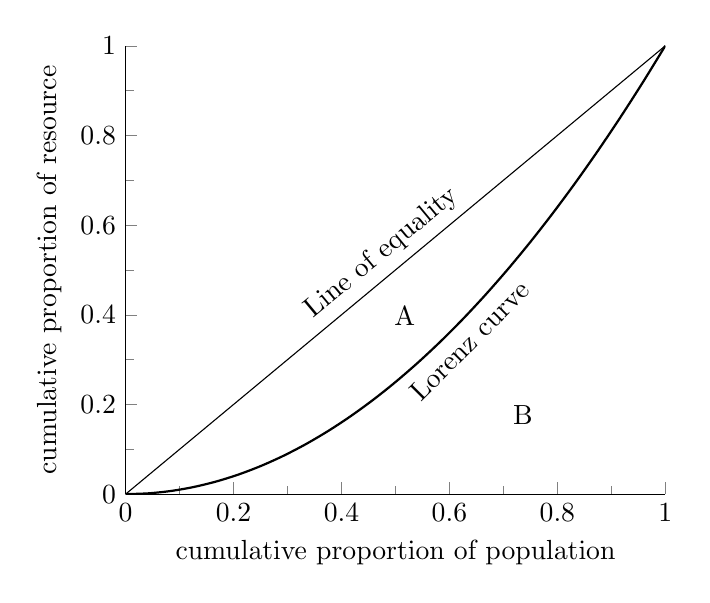
\begin{tikzpicture}
    \begin{axis}[
      xlabel = {cumulative proportion of population},
      ylabel = {cumulative proportion of resource},
      axis y line*=left,
      axis x line*=bottom,
      minor tick num=1,
      xmin = 0,
      xmax = 1,
      ymin = 0,
      ymax = 1
    ]
    \addplot[domain=0:1]{x} node[midway,above,sloped]{Line of equality};
    \node[anchor=north west] at (0.48,0.44) {A};
    \node[anchor=north west] at (0.7,0.22) {B};
    \addplot[domain=0:1,smooth, thick, label=$x$]{x^2}
      node[midway,below,sloped]{Lorenz curve};
    \end{axis}
\end{tikzpicture}

While the area under a curve is commonly calculated using the Newton-Leibnitz formula \cite{kalinski2016}, in practice it is often simpler to calculate the area under the Lorenz Curve as the sum of a the area of a series of trapeziums, correlating in width to the unit interval being measured.  Using this approach, the Gini Index can be calculated as:

\[G=1-\sum_{i=1}^{n}\left[ \left( q_{i}+q_{i-1} \right) \left( p_{i}-p_{i-1} \right) \right]\]

where \textit{q} is the cumulative proportion of the distribution (i.e. wealth / income) and \textit{p} is the cumulative proportion of the population with ownership of control over that portion of the total distribution.  A detailed explanation for how this method is arrived at is given by \cite{bellu2006inequality}.
The Gini index gives us a value of between 0 and 1, where 0 indicates perfect equality of distribution of resources within the population, and 1 is total inequality, i.e. one single entity controls all the 100\% of resources.

\subsection{Atkinson Index}

The Gini Index is useful as a base for calculating inequality, but it has limitations in describing the qualities of inequality.  As the Gini Index is based on the ratio of total areas under the curve, it does not account for variance or skewness, and it also means that two different distributions can potentially have the same Gini index, which could potentially affect the tracking of changes over time.

For this reason, our model employs the Atkinson index \cite{atkinson1970measurement} as a further measure of decentralization to allow us to cross-reference our Gini index against a measurement that can be fine-tuned to our requirements, and which can be used to capture the any nuance in distribution of different measurements.

The Atkinson index is based on the social-welfare approach, which at a high level tracks the amount of resources that would need to be redistributed to achieve a certain level of equality.

\[A(\varepsilon) = 1 - \left(\frac{1}{N} \sum_{i=1}^{N} \left(\frac{y_i}{\mu}\right)^{1 - \varepsilon}\right)^{\frac{1}{1 - \varepsilon}}, \quad \quad \varepsilon \neq 1
\]

\[A\left( \varepsilon \right)=1-\frac{\prod_{i=1}^{N}\left( y_{i}^{\frac{1}{N}} \right)}{\bar{y}}, \quad \quad \varepsilon=1\]

where the parameters include:

\begin{center}
\begin{tabular}{|l|l|}
\hline
$\epsilon$ & inequality aversion parameter where $\epsilon>0$ \\ \hline
$n_{i}$ & number of people in the ith income group \\ \hline
N & total number of people \\ \hline
$y_{i}$ & average income of the ith income group \\ \hline
$\mu$ & average income of the total population \\ \hline
\end{tabular}
\end{center}

The Atkinson index is very closely linked to the generalized entropy index, and other related entropy based indices, such as the Theil index (i.e. GE(1)).

\subsection{Herfindahl-Hirschman Index}

The Herfindahl-Hirschman Index is commonly used as a measurement of competition within a certain industry sector. It has found applications in regulation where antitrust authorities \cite{usdoj2015}. It is calculated as the sum of the square of the percentage market share of each entity.

As the HHI is based on percentage shares of the market, it becomes close to zero for a market that has been commoditized, having a large number of participants with a relatively equal share.  Conversely, the HHI approaches 10,000 for a highly concentrated market, with 10,000, or $1 \times 100^2 $, being a single entity monopoly.

Our model adapts the standard HHI by re-scaling it to make it comparable with other indices employed in the model, by dividing the HHI by $10^4$ so that it falls in the interval $0 <= HHI <= 1$. As such, the re-scaled HHI, denoted by $\theta$, is expressed via the following formula, where $n$ is the total number of participants in the market, $P$ is the total number of units produced in the entire market, and $p_i$ is the number of units consumed from $i^{th}$ participant.

\[\theta = \sum_{i=1}^{n} \frac{(p_{i}/P*100)^{2}}{10^{4}}
\]

As an example, in measuring concentration in the block building market, $P$ would be the total number of blocks produced in an interval,  $p_i$ would be the blocks proposed to the network that are built by the $i^{th}$ block builder.

The US DoJ generally classifies markets within three discrete categories \cite{usdoj2015}:

\begin{center}
\begin{tabular}{|l|l|}
\hline
Unconcentrated & $HHI < 1,500$  \\ \hline
Moderately Concentrated & $1,500 <= HHI <= 2,500$ \\ \hline
Highly Concentrated & $HHI > 2,500$ \\ \hline
\end{tabular}
\end{center}

Because the Herfindahl-Hirschman Index is commonly used for identifying and measuring the presence of monopolies in industry, it is more suited to the data-points in our model that measure the infrastructure that is provide as a service or public good by a relatively small number of actors, as opposed to measuring the distribution of ownership or control of some asset.  This makes it particularly useful for merging middleware such as block builders or relays.

\subsection{Shannon Index}

The Shannon Index \cite{shannon1998mathematical} is part of a family of measurements that are derived from information theory and which are based on concept of entropy.  Other measurements in this category include the Generalized Entropy measurement, and the Theil indices.

The Shannon index is a measure of the amount of entropy in a data set.  It was intended to be used to measure the amount of information content in a signal, where information content can be considered as a measurement of the unexpectedness of a particular value occurring at a specific point in the signal, and entropy is the \textit{average} level of unexpectedness within a signal.  

Shannon gives examples of strings of characters, where the more characters and randomness there is, the lower the probability of predicting the next character in the string, and the more unexpected it is when that value occurs as predicted.  The less often the next character can be predicted correctly, the higher the entropy.  A basic example of this concept is a coin toss, where one party chooses heads, where there is a 50\% chance of the expected value (i.e. heads) occurring as predicted.  As this has a relatively high probability, $p(heads) = 0.5$, coin tosses have low entropy. If we roll a die, the entropy increases and the probability of an expected value decreases, i.e. $p(6) = 0.16$.

Entropy as applied within the field of economics was systematized by Theil \cite{theil1967economics}, and has found application in measuring inequality within a distribution of resources, and later within several studies of decentralization in cryptocurrencies \cite{zhang2022sok, gochhayat2020measuring, kusmierz2022centralized}.

The Shannon index is commonly expressed using the following formula, where $p_{i}$ is the amount of resources allocated to the $i^{th}$ entity in the population in proportion to the total amount of resources.
\[H' = - \sum_{x} p(x) \log_{2} p(x)\]
The Shannon index was designed for use with categorical data, as opposed to continuous data, for which the  GE index is better suited \cite{tran2021harnessing}.   However, for the purposes of measuring distribution of native asset (i.e. ETH), we have applied the Shannon index to ranges of amounts of ETH.  In this context, $p_i$ is the proportion of the asset owned by the $i^{th}$ percentile of the population.

The Shannon index has a range between 0 and the logarithm of the number of categories in the dataset, i.e. $0<=H'<=log(n)$.  The more centralized a system becomes, the closer the Shannon index will be to zero \cite{kusmierz2022centralized}.

\subsection{Tail Ratios}

According to Atkinson \cite{atkinson1970measurement}, the Gini index is affected by changes closer to the median of the distribution more than it is affected by changes at tail ends of the distribution.  In order to account for this characteristic of the Gini index, we employ a series of tail ratios to highlight any changes in the shape of the distribution that affect the lower and upper percentiles.

Our model incorporates the Palma Ratio \cite{palma2011homogeneous}, which is the ratio of the share of resources allocated to the top 10\% of the distributed to the lower 40\% of the distribution.  Palma concludes that changes in the level of inequality tend to happen more at either end of the distribution, with the middle being affected less.  We complement the Palma ratio with several other inter-decile ratios such as P90:P10, P50:P10, P80:P20 (Pareto Ratio).

These ratios are employed simply as a complement to the other indices in our model, as a method of identifying potential areas where the model may need to be fine-tuned to correctly track changes over time.  By themselves they are not useful measurements as the range within the results are not bounded, as with the Gini index, or Herfindahl-Hirschman Index.

\subsection{Euclidean Distance}

As we are interested in measuring the changes to levels of decentralization over time, we employ the Euclidean Distance measurement of a way to track changes over discrete intervals.  In order to do this, we apply the Euclidean Distance measurement to the allocation of resources to either single entities or discrete ranges of asset ownership depending on the data set, from one interval to the following interval.

As we are derive a set of Euclidean Distances for each interval, we are particularly looking at the maximum distance that occurs between two intervals.  As such, we adapt the Euclidean Distance formula in our model to derive the maximum ED per measurement dimension per interval, using the following formula:

\[ED = \max \left( \sqrt{\sum_{i=1}^{n} (x_{i,2} - x_{i,1})^2} \right)
\]

The Euclidian Distance, as well as well similar measurements have been employed in previous research of decentralization in blockchain networks in previous studies \cite{gochhayat2020measuring}, in relation to measuring governance in decentralized networks, where our model employs this measurement as a means to identifying changes to decentralization over time.

\vspace{12pt}

\printbibliography

\end{document}
